% Fig. 2 of the report: what a simulated data point looks like.
% The table values are the first four training patients of dataset 0, scenario A, rounded to
% 2 decimals: rtds.simulate.simulate_dataset(cfg, 0, rho, "A").train, rows 0-3, at rho = 0 and 0.9.
% Build: pdflatex fig_datapoint.tex  ->  fig_datapoint.pdf (vector, upload to Overleaf)
\documentclass[border=2pt]{standalone}
\usepackage[scaled]{helvet}
\renewcommand\familydefault{\sfdefault}
\usepackage{tikz}
\usepackage{booktabs}
\usetikzlibrary{arrows.meta}
\definecolor{SUBlue}{HTML}{002F5F}
\definecolor{SUSky}{HTML}{ACDEE6}
\definecolor{SUFire}{HTML}{D95E00}
\begin{document}
\begin{tabular}{@{}c@{}}
  % Timeline of one patient
  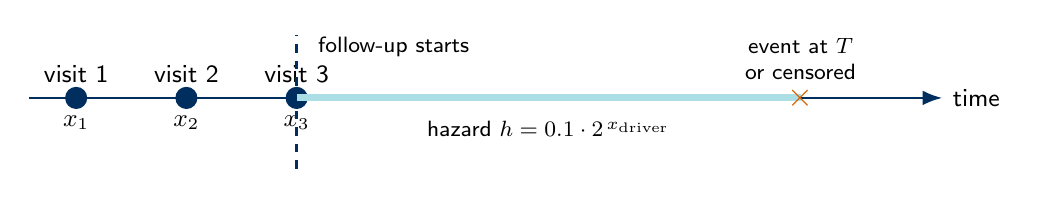
\begin{tikzpicture}[x=1cm, y=1cm, font=\small]
    \draw[-{Latex[length=2.5mm]}, line width=0.9pt, SUBlue] (0, 0) -- (11.6, 0) node[right, text=black] {time};
    \foreach \x/\k in {0.6/1, 2.0/2, 3.4/3} {
      \fill[SUBlue] (\x, 0) circle (4pt);
      \node[above=2pt] at (\x, 0) {visit \k};
      \node[below=3pt] at (\x, 0) {$x_{\k}$};
    }
    \draw[line width=0.9pt, SUBlue, dashed] (3.4, -0.9) -- (3.4, 0.8);
    \node[anchor=west, font=\footnotesize] at (3.55, 0.65) {follow-up starts};
    \draw[line width=2.5pt, SUSky] (3.4, 0) -- (9.8, 0);
    \node[font=\large\bfseries, text=SUFire] at (9.8, 0) {$\times$};
    \node[above=3pt, align=center, font=\footnotesize] at (9.8, 0) {event at $T$\\or censored};
    \node[below=5pt, font=\footnotesize] at (6.6, 0) {hazard $h = 0.1 \cdot 2^{\,x_{\mathrm{driver}}}$};
  \end{tikzpicture}\\[4pt]
  % Four simulated patients at two correlation levels (driver = visit 3, in bold)
  {\footnotesize
  \begin{tabular}{@{}c ccc ccc rl@{}}
  \toprule
  & \multicolumn{3}{c}{$\rho = 0$} & \multicolumn{3}{c}{$\rho = 0.9$} & \multicolumn{2}{c}{Follow-up} \\
  \cmidrule(lr){2-4}\cmidrule(lr){5-7}\cmidrule(l){8-9}
  Patient & visit 1 & visit 2 & \textbf{visit 3} & visit 1 & visit 2 & \textbf{visit 3} & time & outcome \\
  \midrule
  1 & $-$0.93 & 0.19 & \textbf{$-$0.38} & $-$0.75 & $-$0.46 & \textbf{$-$0.38} & 0.22 & event \\
  2 & 0.66 & $-$2.11 & \textbf{0.75} & 0.96 & 0.00 & \textbf{0.75} & 8.41 & censored \\
  3 & 0.85 & $-$0.54 & \textbf{0.13} & 0.49 & 0.09 & \textbf{0.13} & 19.29 & censored \\
  4 & 0.65 & 1.56 & \textbf{0.52} & 0.76 & 1.21 & \textbf{0.52} & 0.71 & event \\
  \bottomrule
  \end{tabular}}
\end{tabular}
\end{document}
